\chapter{Aerodynamic Design}
\label{ch:AerodynamicDesign}
This chapter delves deeper into the design of wing and fuselage subsystems.
The empennage will be discussed in \Cref{ch:Stability_and_Control}, because it is mainly dependent on stability characteristics.
Since many dependencies and iterations influence the wing and fuselage design, this chapter will discuss the methods of designing these subsystems, and each section will end with an overview of the final parameters after the iteration of all subsystems.

\section{Wing Configuration}
Three different wing configurations are possible for the vehicle: low-wing, mid-wing or high-wing.
Each configuration has its advantages and disadvantages, and therefore, a trade-off needs to be made between the three configurations.
The low-wing configuration immediately drops out because the rotors would collide with the fuselage during vertical ascent since the wings are folded, and the ground footprint limits to place the engines more outward. 
For the mid-wing configuration, this same principle holds.
From historical data, a taper ratio of \num{0.4}~\cite{ADSEEIslides} was taken and the fact that three engines are mounted on the wing, the propellers would collide with the fuselage.
Therefore, the vehicle will have a high-wing configuration.
This allows placing the fuselage closer to the ground, making payload loading easier.
Moreover, the propellers will have more ground clearance and do not collide with the fuselage~\cite{raymer1992aircraft}.

\section{Wing Planform}
During the preliminary sizing, the surface area of the wing was calculated using class I and class II estimations.
From this, the wing sizing and shaping can be conducted.
Since the vehicle is set to have a cruise speed of \qty{200}{km/h}, the vehicle will fly with Mach numbers in the subsonic regime.
Hence, it can be assumed, from historical data that the quarter chord sweep, $\Lambda_{c/4}$, is zero and that the taper ratio, $ \lambda$, is equal to \num{0.4}~\cite{ADSEEIslides}.
From the surface area, $S$, span, $b$, and taper ratio, $\lambda$, the root and tip chord, $c_\text{r}$ and $c_\text{t}$ can be calculated in \Cref{eq:rootcrd,eq:tipcrd}, respectively.
After finding the root chord ($c_{r}$), the Mean Aerodynamic Chord (MAC) is calculated using \Cref{eq:MAC}.
The $y$-location of the MAC ($y_{MAC}$) can be retrieved using the taper ratio and wing span in \Cref{eq:ymac}.
Moreover, the leading-edge sweep ($\Lambda_{LE}$) is calculated using the quarter chord sweep angle, taper ratio and the aspect ratio in \Cref{Sweep_LE}.


\begin{minipage}{.45\linewidth}
    \begin{equation}
        \label{eq:rootcrd}
        c_\text{r} = \frac{2S}{(1+\lambda)b}
    \end{equation}
    \begin{equation}
        \label{eq:tipcrd}
        c_\text{t} = c_\text{r} \lambda
    \end{equation}
    \begin{equation}
        \label{eq:MAC}
        \mathrm{MAC} = \frac{2}{3}c_\text{r} \left( \frac{1+\lambda+\lambda^2}{1+\lambda} \right)
    \end{equation}
    
\end{minipage}
~
\begin{minipage}{.45\linewidth}
    
    \begin{equation}
        \label{eq:ymac}
        y_\mathrm{MAC} = \frac{b}{6} \left( \frac{1+2\lambda}{1+\lambda}\right )
    \end{equation} 
    \begin{equation}
    \label{Sweep_LE}
        \Lambda_{LE} = \tan(\Lambda_{c/4}) + \frac{(1-\lambda)}{A(1+\lambda)}
    \end{equation}
\end{minipage}\\

The values for the wing platform design, obtained from the equations, can be visualised in \Cref{tab:wing_planform}.
The dihedral angle, $\Gamma$, was chosen for a high-wing configuration with unswept wings obtained from historical data from \textcite{raymer1992aircraft}. The final wing geometry can be visualised in \cref{fig:WingPlanform}.



\begin{table}[h]
  \hspace{-0.75cm}
  \begin{minipage}{0.75\textwidth}
    \centering
    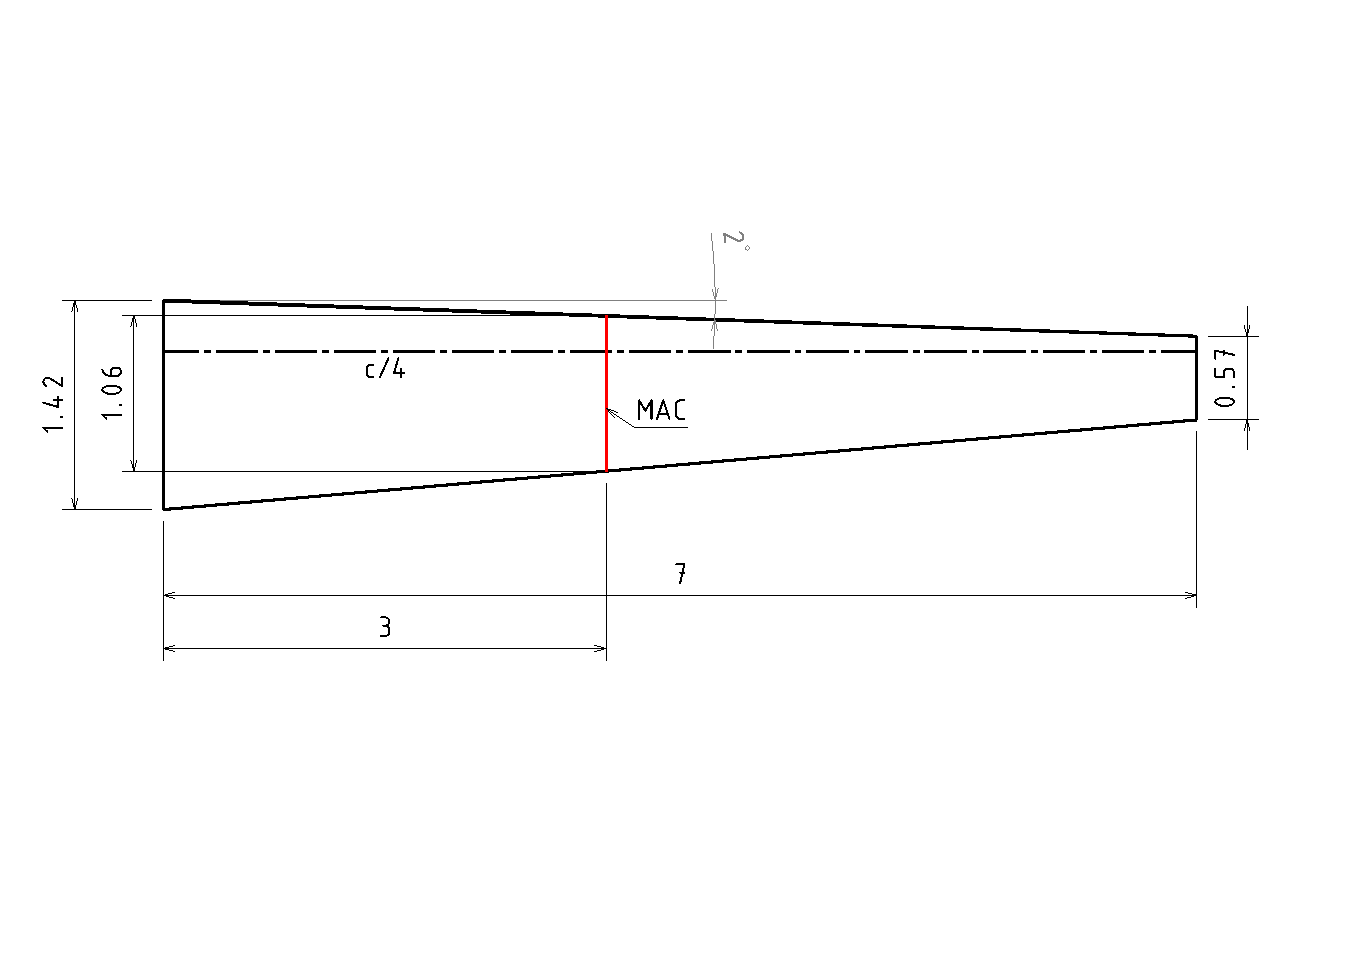
\includegraphics[width=1\linewidth]{figures/WingPlanform}
    \captionof{figure}{Top view of half wing with MAC highlighted}
    \label{fig:WingPlanform}
  \end{minipage}
  \begin{minipage}{0.2\textwidth}
    \centering
    \caption{Wing platform design values}
    \label{tab:wing_planform}
    \begin{tabular}{
        @{}
            >{$}l<{$}
        |S[table-format=2.2]
            >{\collectcell\unit}l<{\endcollectcell}
        @{}
    }
        \toprule
        S                 & 14            &  m^2        \\
        b                 & 14            &  m          \\
        A                 & 14            &  -          \\
        c_\text{r}        & 1.42          &  m          \\
        c_\text{t}        & 0.57          &  m          \\
        \mathrm{MAC}      & 1.06          &  m          \\
        y_\mathrm{MAC}    & 3.0           &  m          \\
        \Lambda_{c/4}     & 0             &  deg        \\
        \Lambda_{LE}      & 2             &  deg        \\
        \lambda           & 0.4           &  -          \\
        \Gamma            & 1             &  deg        \\
        \bottomrule
    \end{tabular}
  \end{minipage}
\end{table}


\section{Airfoil Selection}
\label{sec:Airfoil_Selection}
After the wing planform has been fixed, it is crucial to select an airfoil which is fit for the mission requirements.
Literature research was performed on airfoils used for similar eVTOL designs as well as reference aircraft, which operate at similar velocities to the \textit{Swing} while carrying a similar payload mass.
The airfoil selection was performed keeping in mind the fact that the vehicle shall operate at a low altitude, leading to a high Reynolds number due to increased density:

\begin{equation}
    \label{eq:reynolds}
    Re = \frac{\rho V l}{\mu} 
\end{equation}

In this equation, $\rho$ represents the density at cruise altitude, $V$ the velocity, $l$
describes the characteristic length,
which in the case of aircraft wings, can be considered to be the mean aerodynamic chord length (MAC).
Finally, $\mu$ is the dynamic viscosity of air, which can be estimated from the International Standard Atmosphere (ISA).
At a cruise altitude of $h=\qty{500}{\m}$, $\mu=\qty{1.77e-5}{\kg\m\per\s}$.

Using \Cref{eq:reynolds}, a Reynolds number of \num{4.0e6} is calculated, which is used in the airfoil analysis.
Based on this particular Reynolds number, a selection of airfoils was performed that shall then be analysed in further detail and traded off.
Hence, the following six different airfoils were considered in the airfoil trade-off~\cite{Prelim_airfoil,Eppler423,eppler1990airfoil}:
\begin{multicols}{2}
\begin{itemize}
    \item NASA Langley LS(1) 0417
    \item NACA 4416
    \item NACA 4412
    \item Eppler 423
    \item Eppler 560
    \item Eppler 562
\end{itemize}
\end{multicols}
After the airfoil selection, the trade-off criteria should be established for the final design choice.
While the airfoils can only be analysed based on their technical parameters, it is important to consider the mission requirements when selecting the airfoil.
Therefore, a list of criteria was compiled, with each criterion being allotted importance on a scale from one to three.
Afterwards, each criterion was translated into technical parameters based on the relative importance of each parameter in each of the criteria.
The values for each parameter were then summed up and converted into percentages, enabling setting-up a technical trade-off for the airfoil selection.
The criteria considered, as well as the final importance determined for each technical parameter, shall be presented in \Cref{tab:crit_airfoil}.

\begin{table}[h]
\caption{Airfoil criteria}
\label{tab:crit_airfoil}
\sisetup{table-format=2}
\resizebox{\columnwidth}{!}{%
\begin{tabular}{S[table-format=1]l|SSSSSS}
\toprule
\textbf{Importance} & \textbf{Criteria}                    & $C_{\text{l}_0}$ & $C_{\text{d}_{\min}}$ & $C_\text{l}/C_{\text{d}_{\max}}$ & $C_{\text{m}_0}$ & $t/c$ & $\alpha_\text{stall}$ \\
\midrule
2                   & Structural Weight                      &              &       &               &              & 3   &             \\
3                   & Power required                       &              & 3     & 2             &              & 1   &             \\
1                   & Stability                            &              &       &               & 3            &     & 1           \\
2                   & High lift                            & 3            &       & 2             &              & 1   &             \\
2                   & Safety                               &              &       &               & 1            & 2   & 2           \\
                    & \textbf{Design Parameter Importance} & 6            & 9     & 10            & 5            & 15  & 5           \\
                    & \textbf{Percentage}                  & 12           & 18    & 20            & 10           & 30  & 10          \\
\bottomrule
\end{tabular}%
}
\end{table}

It is important to note that, as can be seen in the trade-off, when determining the importance of the parameter, the value of the importance of the criteria was multiplied by the relevance of the criteria before summing up to obtain the final score.
Thus, the aforementioned percentages shall be used to score each of the proposed airfoil configurations.
Additionally, the relevance of each of the technical parameters for the airfoil trade-off shall be briefly explained below:

\begin{itemize}
    \item $C_{\text{l}_0}$: The higher the lift coefficient at zero angle of attack, the higher the efficiency for cruise.
    \item $C_{\text{d}_{\min}}$: The lower the minimum drag of the airfoil, the more efficient cruise will be.
    \item $C_\text{l}/C_{\text{d}_{\max}}$: The higher the value, the better, the more range and higher efficiency for the cruise.
    \item $C_{\text{m}_0}$: The more negative the {$C_{\text{m}_0}$} value, the better the controllability for the aircraft will be
    \item $t/c$: A high t/c ratio reduces the structural weight, increases the lift and increases available space for battery storage if required.
    \item $\alpha_\text{stall}$: The stall characteristics depend on the stall angle of the airfoil.
    During transition, stall is not desired.
    However, the angled thrust will counteract this; therefore, the weight is low.
\end{itemize}

In order to compare the technical performance of the aforementioned selected airfoils, specialised software such as XFOIL should be used. This software requires an airfoil shape, of which the data can be obtained from an airfoil database provided by the TU Delft that then can be used as input for the XFOIL and XFLR5 software~\cite{airfoildatabase}.
The airfoils were analysed for each of the criteria stated above using XFOIL and XFLR-5, set at a Reynolds number of \num{4.0e6} and a Mach number of \num{0.16}, which is obtained from the cruise speed requirement.
The results can be seen in \Cref{tab:Airfoil_analysis}.

\begin{table}[H]
    \centering
    \caption{Airfoil parameter values at $\mathrm{Re}=$\num{4.0e6} and $M=$\num{0.16}}
    \label{tab:Airfoil_analysis}
    \begin{tabular}{l|S[table-format=1.2]S[table-format=1.4]S[table-format=3]S[table-format=+1.2]S[table-format=2.1]S[table-format=2]}
        \toprule
        & $C_{\text{l}_0}$ & $C_{\text{d}_{\min}}$ & $C_{\text{l}}/C_{\text{d}_{\max}}$ & $C_{\text{m}}$ & $t/c$ & $\alpha_{\text{stall}}$ \\
        \midrule
        \textbf{LS(1)-0417} & 0.55 & 0.0047 & 120 & -0.12 & 17 & 18 \\
        \textbf{NACA4412} & 0.47 & 0.0088 & 120 & -0.10 & 12 & 14 \\
        \textbf{NACA4416} & 0.51 & 0.0061 & 168 & -0.10 & 16 & 17 \\
        \textbf{E560} & 0.72 & 0.0061 & 162 & -0.17 & 16 & 16 \\
        \textbf{E562} & 0.61 & 0.0057 & 160 & -0.15 & 15 & 17 \\
        \textbf{E423} & 1.16 & 0.0064 & 220 & -0.25 & 12.5 & 14 \\
        \bottomrule
    \end{tabular}
\end{table}

Based on the aforementioned airfoil technical parameters, the airfoils were then scored for each criterion on a range from one to five.
Subsequently, the scores were added up based on the weight of each parameter, leading to the final airfoil choice
\Cref{table:airfoil_scores}.


\begin{table}[h]
\caption{Airfoil trade-off}
\label{table:airfoil_scores}
\centering
\sisetup{table-format=1.1}
\resizebox{\textwidth}{!}{%
\begin{tabular}{S[table-format=2]l|SSSSSS}
\toprule
\textbf{Weight} & \textbf{Parameter} & \textbf{LS(1)-0417} & \textbf{NACA 4412} & \textbf{NACA 4416} & \textbf{E560} & \textbf{E562} & \textbf{E423} \\ \midrule
12 & $C_{\text{l}_{0}}$ & 2 & 1 & 2 & 4 & 3 & 5 \\ 
18 & $C_{\text{d}_{\min}}$ & 5 & 1 & 3 & 3 & 4 & 2 \\ 
20 & $C_\text{l}/C_{\text{d}_{\max}}$ & 1 & 1 & 4 & 4 & 4 & 5 \\
10 & $C_\text{m}$ & 2 & 2 & 2 & 4 & 3 & 5 \\
30 & $t/c$ & 5 & 1 & 4 & 4 & 3 & 1 \\
10 & $\alpha_\text{stall}$ & 5 & 2 & 4 & 4 & 4 & 2 \\ \midrule
\textbf{} & \textbf{Final Score} & \textbf{3.5} & \textbf{1.2} & \textbf{3.4} & \textbf{3.8} & \textbf{3.5} & \textbf{3.0} \\ \bottomrule
\end{tabular}
}
\end{table}

From \Cref{table:airfoil_scores}, it can be seen that the E560 wins the trade-off.
However, the airfoil final scores are in a close range compared to each other, therefore a sensitivity analysis was conducted.
Firstly, each parameter was removed separately, and the final score was analysed.
The E560 won five out of six times, meaning the weights are robust.
The winner in each of the cases, as well as the final score, is presented in \Cref{tab:Airfoil_sensitivity}.
Secondly, the weights were adjusted by $\pm 5\%$ In all cases; the E560 won the trade-off.
The airfoil shape is presented in \Cref{fig:Airfoil_drawing}.
\begin{table}[H]
    \centering
    \caption{Airfoil sensitivity analysis}
    \label{tab:Airfoil_sensitivity}
\begin{tabular}{l|l}
\toprule
\textbf{Parameter Removed}       & \textbf{Winning Airfoil}                    \\ \midrule
$C_{\text{l}_{0}}$             & E560                               \\
$C_{\text{d}_{\min}}$           & E560                               \\
$C_\text{l}/C_{\text{d}_{\max}}$   & LS(1)-0417                         \\
$C_\text{m}$                 & E560                               \\
$t/c$                     & E560                               \\
$\alpha_\text{stall}$        & E560                               \\
    \bottomrule
\end{tabular}
\end{table}

\begin{figure}[h]
    \centering
    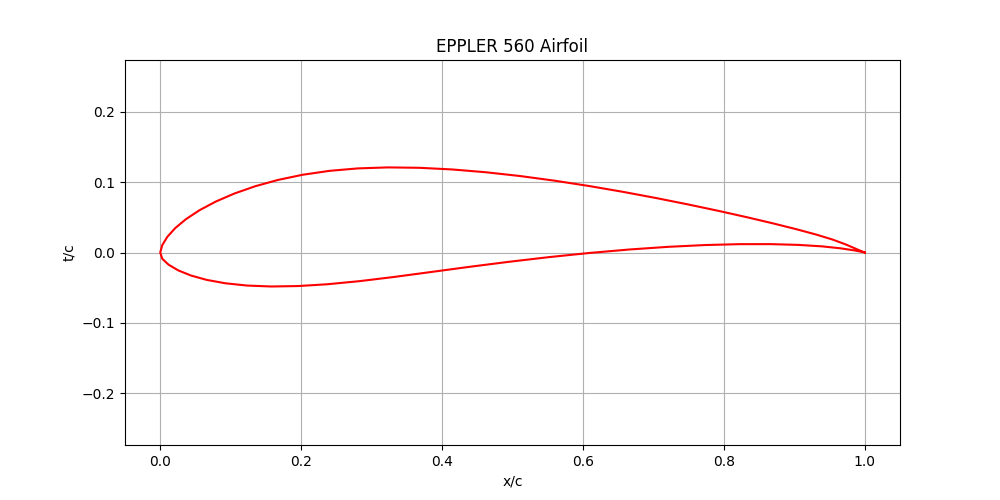
\includegraphics[width=0.5\linewidth]{figures/Airfoiol E560.png}
    \caption{Plot of the Eppler 560 airfoil}
    \label{fig:Airfoil_drawing}
\end{figure}



\section{Fuselage Design}
\label{sec:fuselage_design}
An aircraft’s fuselage has many functions, which all need to be fulfilled by the design.
For this eVTOL concept, the following functions were considered the most important:
\begin{itemize}
    \item Fit the passengers in a comfortable and spacious manner.
    \item Offer load-path for lifting surfaces and landing gear.
    \item Accommodate the layout of electrical and control systems.
    \item Contain easily accessible compartments for luggage. 
    \item Provide easy and quick boarding and disembarking of the aircraft.
\end{itemize}
The first function is chosen to be important since the design is supposed to be a luxurious mode of transportation and thus should provide enough space and comfort.
Furthermore, the fuselage design should aim to keep the fuselage drag at a minimum while still ensuring all the above functions are satisfied.

The first step in designing the fuselage is to look at how the payload will fit inside and, thus, how it will satisfy the first function.
To do this, the following mannequin seen in \Cref{fig:seating_manikin} is used.
It shows the dimensions of the 99th percentile male, meaning that 99\% of the male population will have equal or smaller dimensions.

To keep the cross-sectional area of the fuselage to a minimum, a seating position with the lower legs at 45 degrees was chosen.
To further decrease the cross-sectional area and still take passenger comfort into account, the seats are tilted backwards.
According to \cite{goossens2000biomechanical}, the backrest inclination is comfortable between an angle of 65 and 85, while the seat inclination is comfortable between 5 and 15 degrees; this is confirmed by research by \cite{yao2023sitting}.
To also be comfortable if the aircraft is climbing or descending, a seat inclination of 10 degrees and a backrest inclination of 75 degrees are chosen.
This results in the seated position seen in \Cref{fig:seating_manikin}.


\begin{figure}[!htb]
    \centering
    \begin{minipage}{.5\textwidth}
        \centering
        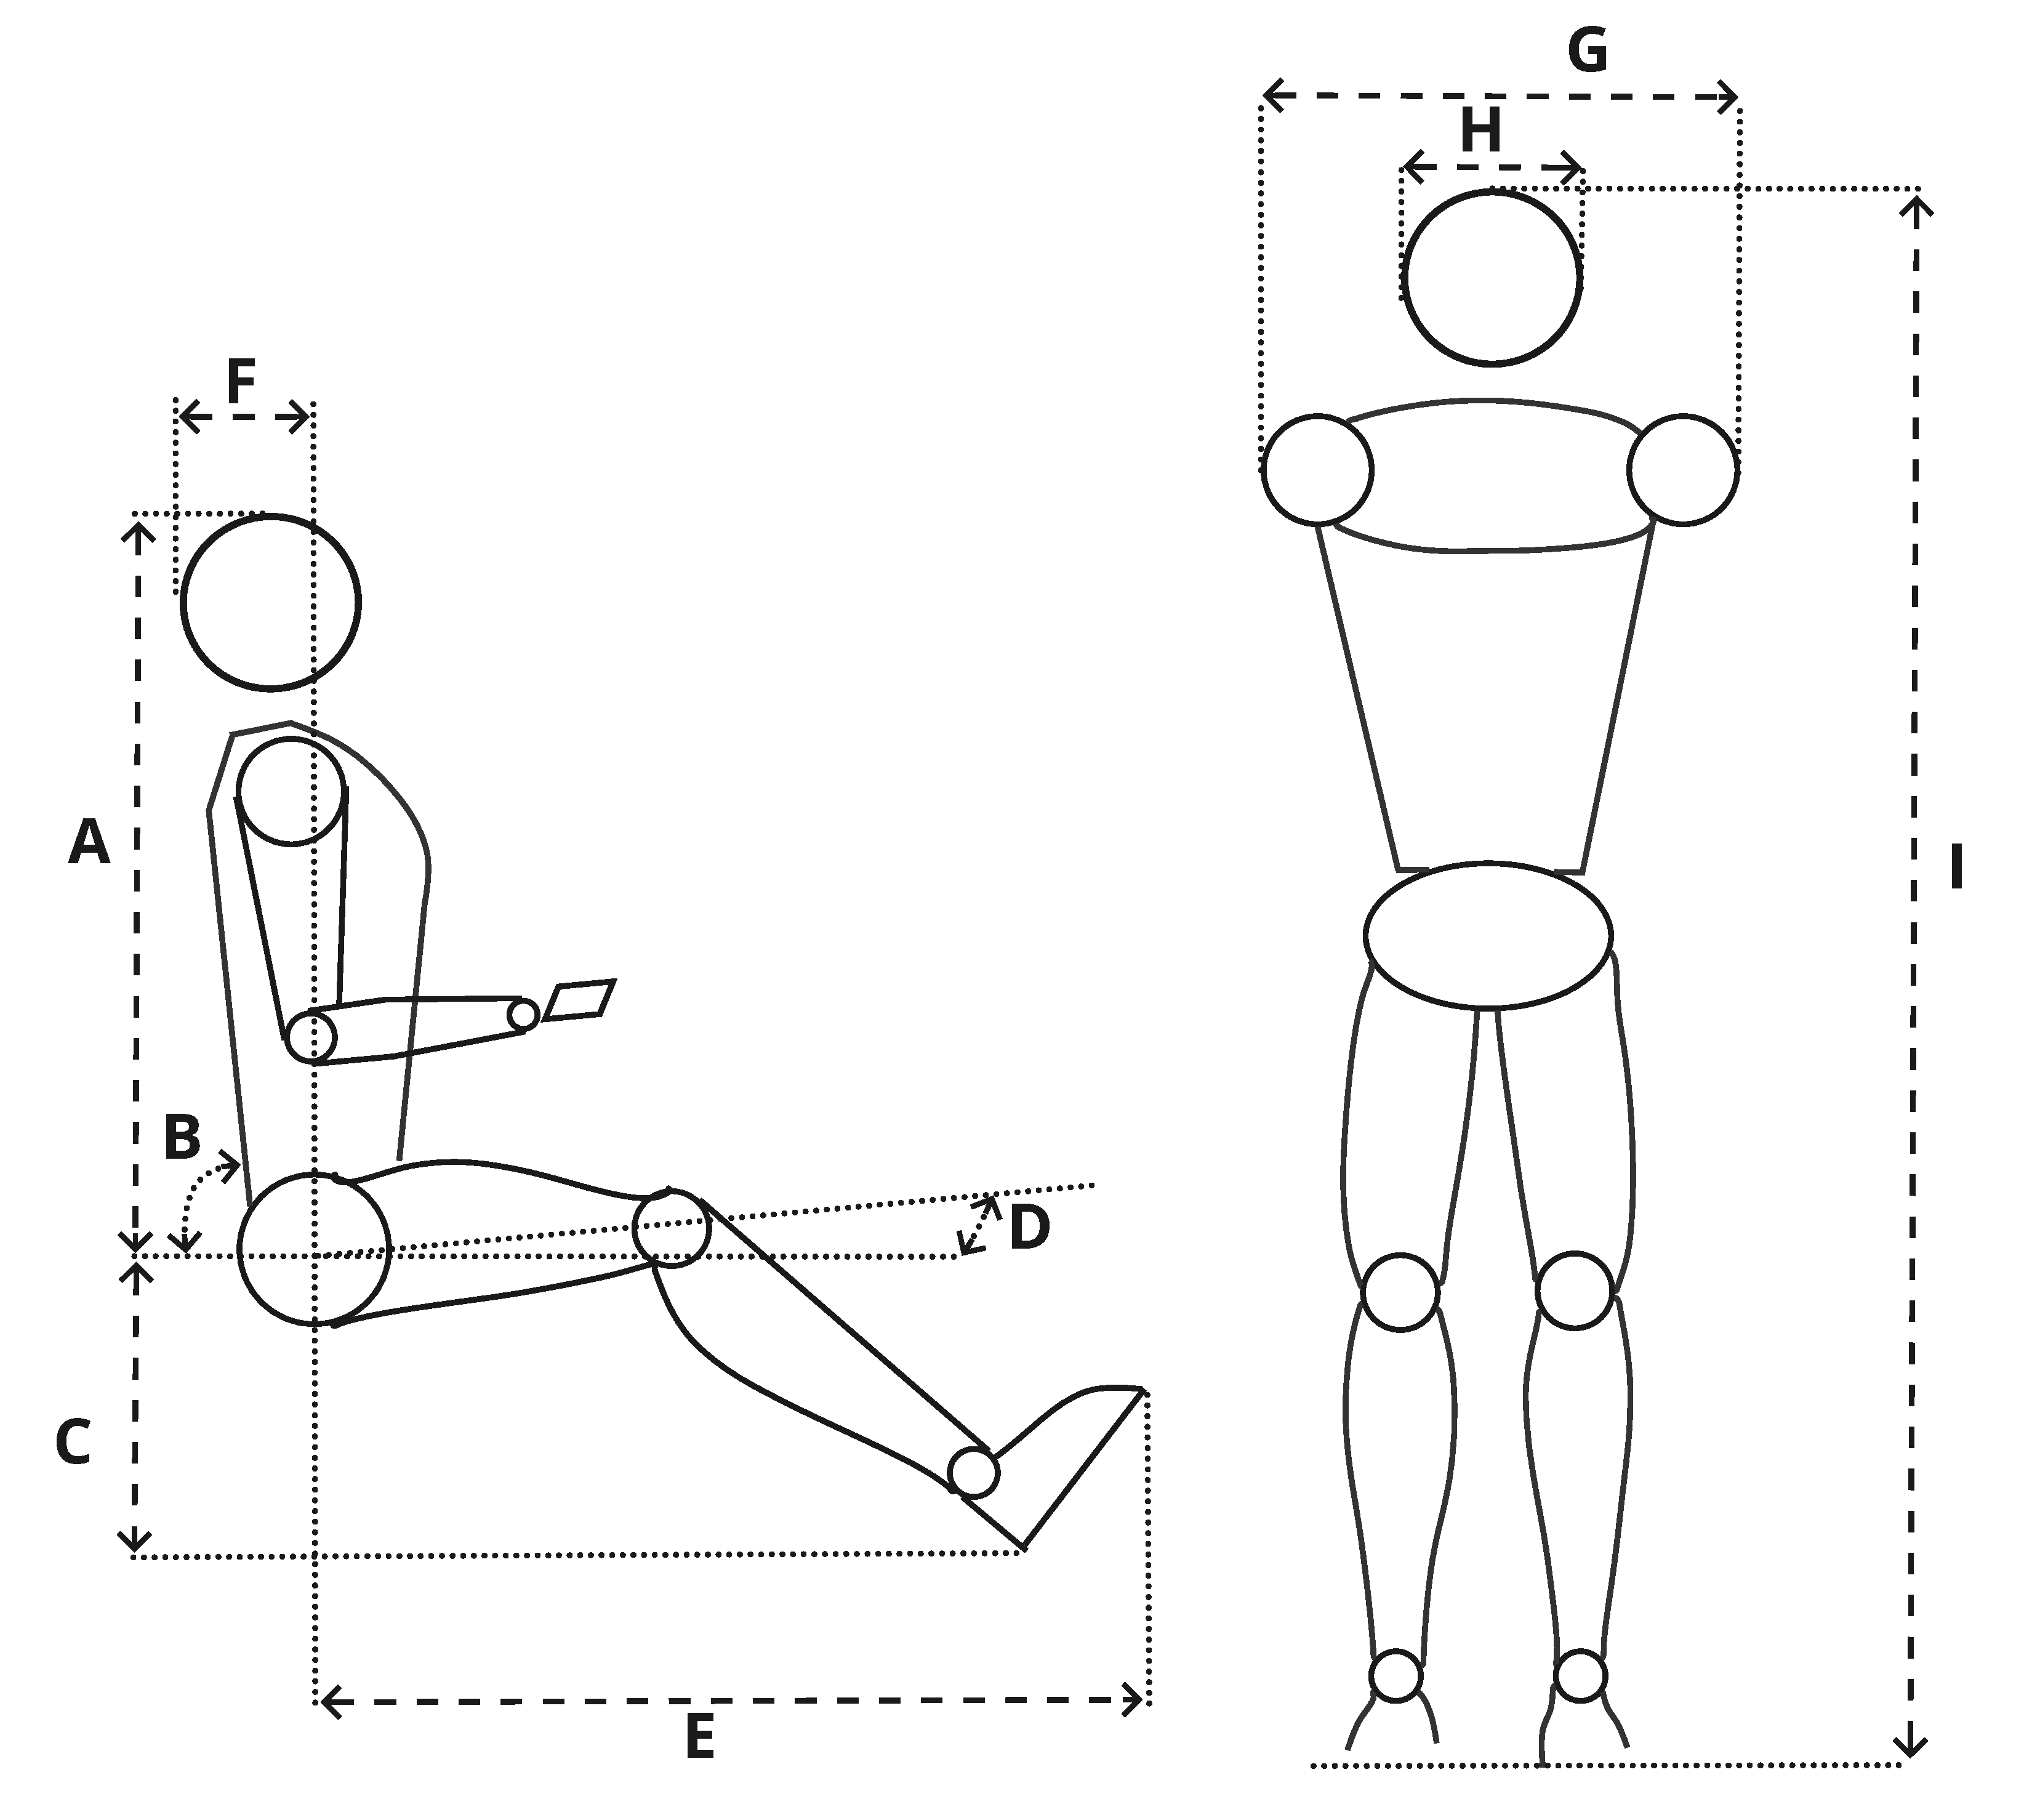
\includegraphics[width=1.0\linewidth]{figures/Fuselage_Manikin}
    \end{minipage}%
    \begin{minipage}{0.2\textwidth}
        \centering
   \begin{tabular}{
       @{}
       l
       |S[table-format=2.2]
           >{\collectcell\unit}l<{\endcollectcell}
       @{}
   }
        \toprule
        A         & 0.85  & m       \\
        B         & 75    & \degree \\
        C         & 0.41  & m       \\
        D         & 10    & \degree \\
        E         & 0.88  & m       \\
        F         & 0.23  & m       \\
        G         & 0.55  & m       \\
        H         & 0.17  & m       \\
        I         & 1.91  & m       \\\bottomrule
        
    \end{tabular}
    \end{minipage}
    \caption{99th percentile male in standing and seating configuration, adapted from \textcite{gudmundsson2013general}.}
    \label{fig:seating_manikin}
\end{figure}

From this seated position, a cross-section of the fuselage can be drawn, which can be seen in \Cref{fig:Fuselage_crosssection}. This cross-section gives an inner diameter and width data from literature~\cite{ADSEEIslides}; it can be concluded that for a non-pressurised composite aeroplane, 5 cm thickness of the fuselage is sufficient, and therefore, the outer diameter of the fuselage is found to be 170 cm.

\begin{figure}[htpb]
    \centering
    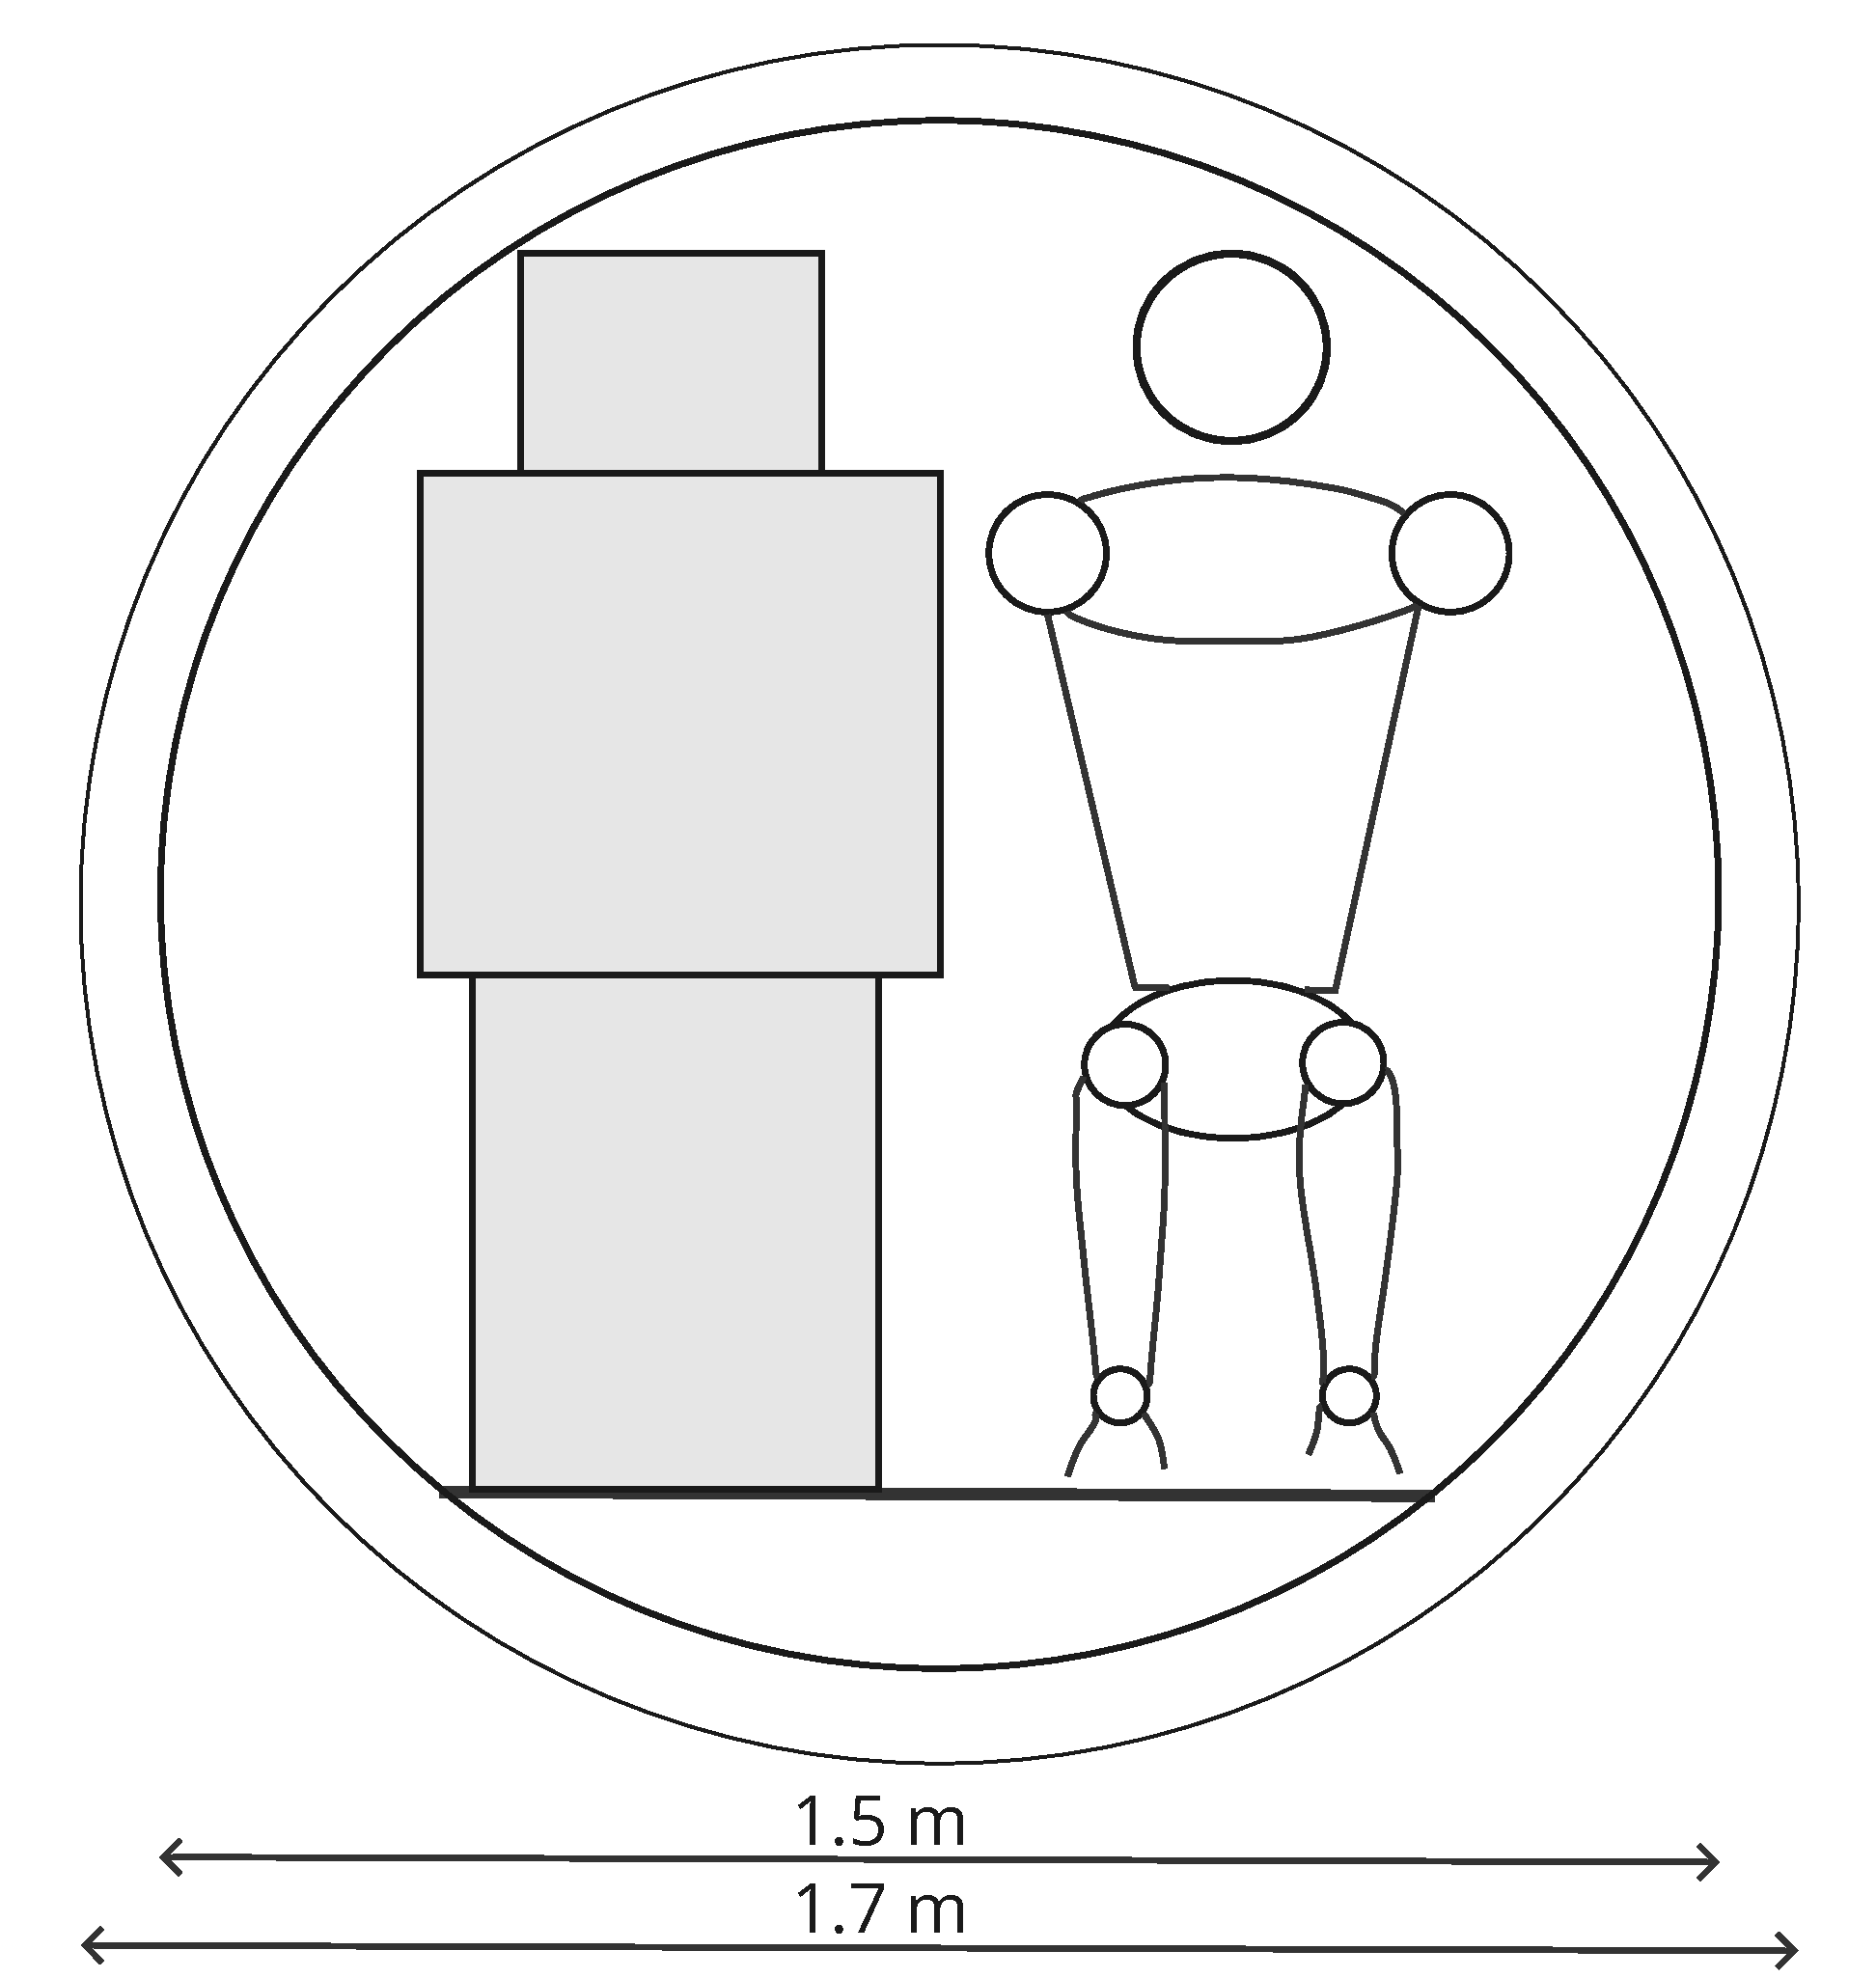
\includegraphics[width=0.5\linewidth]{figures/Fuselage_crossection}
    \caption{Drawing of the fuselage cross-section with passengers loaded}
    \label{fig:Fuselage_crosssection}
\end{figure}

After the cross-section, it is important to look at the longitudinal shape of the fuselage.
Since the aircraft does not need to have a large internal volume, a tadpole fuselage shape was chosen.
The forward part of the fuselage is shaped to sustain a laminar boundary layer and a wetted area of more than 25\%.
This is less than a conventional fuselage \cite{gudmundsson2013general}.
The standard tadpole design, found in almost all sailplanes nowadays, was adapted to fit the \textit{Swing eVTOL}.
The main difference is the decrease in the $l/d$ (length over diameter) ratio since the length of the \textit{Swing} is limited by the ground footprint, and the diameter of the fuselage is bigger since it has two seats abreast.

Due to the wings being next to the aeroplane when in hover configuration, entering the back two seats with a normal door is not a possibility.
The solution to this problem is that the front two seats are on rails such that they can be moved forward.
The rear seats can be boarded via a door at the side of the fuselage in front of the wing.
The final design of the fuselage gives passengers the same amount of comfort as a business class seat in a general aviation aircraft while being smaller in diameter than a \textit{Cessna Citation Ultra}.
The final fuselage design is displayed in \Cref{fig:fuselage_sideview}.

\begin{table}[htpb]
    \centering
  \hspace{-2cm}
  \begin{minipage}{0.75\textwidth}
    \centering
    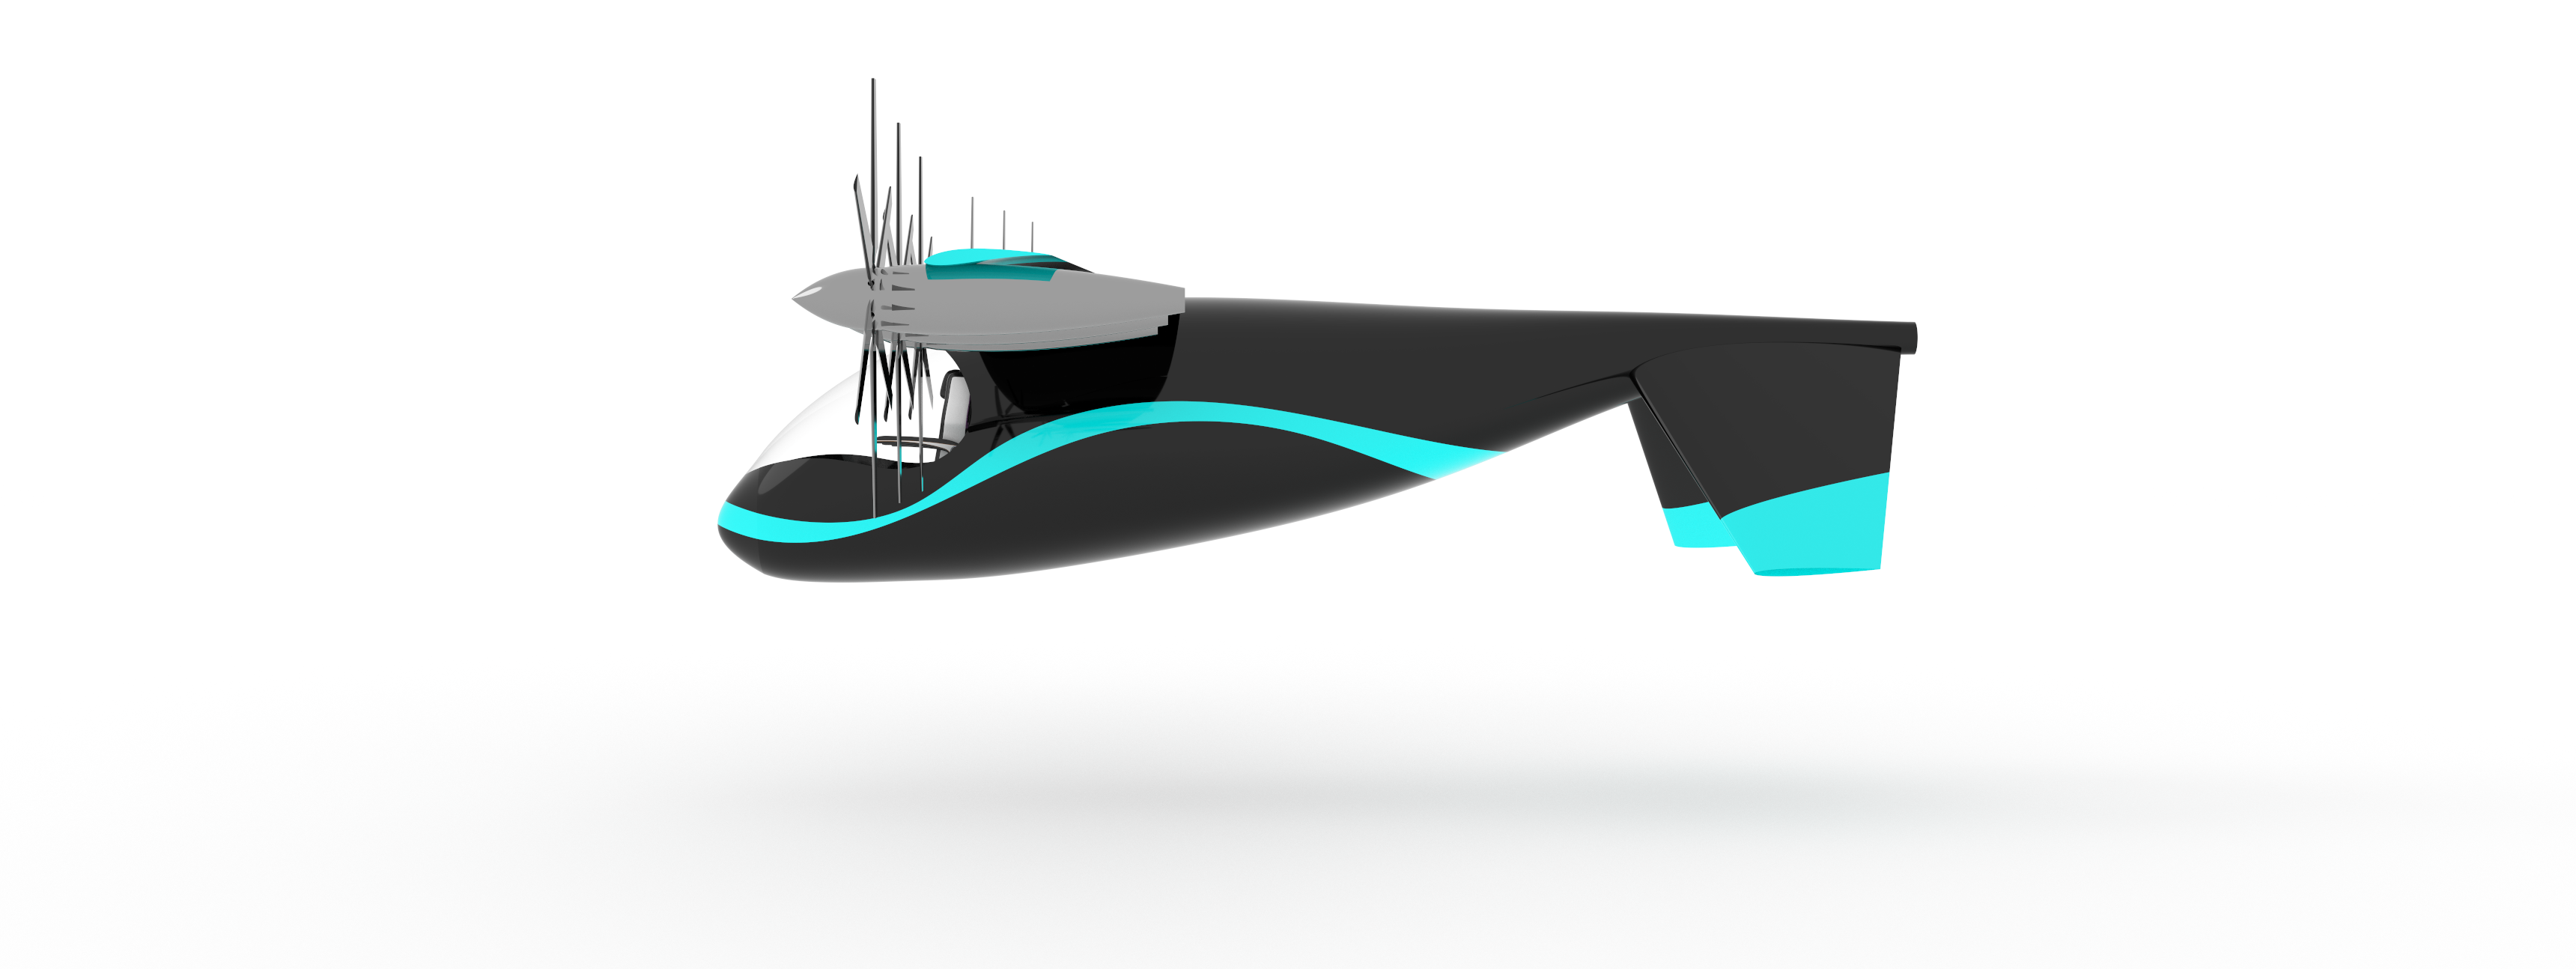
\includegraphics[width=1.2\linewidth]{figures/sidebeauty.png}
        \captionof{figure}{Side view of the fuselage}
    \label{fig:fuselage_sideview}
  \end{minipage}
  \begin{minipage}{0.2\textwidth}
    \centering
    \caption{Fuselage design values}
    \label{tab:fuselage_design}
    \begin{tabular}
    {
        @{}
            >{$}l<{$}
        |S[table-format=1.1]@{\,\unit{\m}}
        @{}
    }
        \toprule
        l_\text{fus}           & 8.0                 \\
        d_\text{inner}         & 1.6                \\
        d_\text{outer}         & 1.7 \\
        \bottomrule
    \end{tabular}
  \end{minipage}
\end{table}
